\section{Theoretical Predictions}
\label{secTheoreticalPredictions}

One of non-baryonic particles that has a non-zero contribution to the matter density in the universe is the {\it neutrino}, which used to be considered an excellent candidate for non-baryonic dark matter~\cite{DM_neutrino}. 
There is a relic neutrino background in the Universe, left over from the Big Bang, similar to the photon CMB. Observation of atmospheric and solar neutrino oscillations have established that neutrino have a mass of $\geq$0.05~eV~\cite{NeutrinoMass_SuperK, NeutrinoMass_SNO}. Laboratory measurements of $\beta$-decay constrain the upper limit on neutrino mass to $<$2.05~eV (95\%~C.L.)~\cite{NeutrinoMass_Weinheimer}. This implies that the total relic density of neutrinos is $<$0.07~\cite{WMAP_5year}, thus they are not abundant enough to be the dominant component of dark mater. The neutrino component of dark matter is called `hot' dark matter: since they travel at relativistic speeds at the time of decoupling, they cannot reproduce the observed large structure in the Universe.

Another dark matter candidate are {\it axions}, light pseudo-scalar elementary particles postulated to resolve the strong CP problem in quantum chromodynamics (QCD)~\cite{CPviolation}. Axions are constrained to be very light, with a mass from 10$^{-6}$~eV to 10$^{-3}$~eV~\cite{AxionBounds}, and are expected to be extremely weakly interacting with ordinary matter, which assumes that they were not in thermal equilibrium in the early Universe. The axion relic density calculation relies on same production mechanism assumptions, which makes it possible to find an acceptable range where all constraints are satisfied. Hence, axions present a possible dark matter candidate~\cite{AxionsRosenberg}, and are being searched in experiments which stimulate the conversion of an axion into a single photon in magnetic field~\cite{AxionSearches}. 

While axions could be an excellent solution to the strong CP problem, their small mass requires that they are produced out of thermal equilibrium. In contrast, the dark matter candidates that originate as thermal relics (a process known as thermal freeze-out), can be explored. 
Shortly after the Big Bang, if production and annihilation rates for specific particles are equal, they are in thermal equilibrium with the rest of the Universe. Once the temperature of the Universe falls below the production threshold for this particle species, production ceases. Additionally, the annihilation rate is suppressed by the expansion of the Universe. The present mass density of particle $\chi$ in the units of particle density is given by~\cite{WIMPnucleusScattering1}:

\begin{equation}
\Omega_{\chi} h^{2} = \frac{m_{\chi} n_{\chi}}{\rho_{c}} \approx \frac{3\times10^{-27} \mathrm{cm^{3}s^{-1}}}{\sigma v}
\end{equation}
where $m_{\chi}$ is the particle mass, $n_{\chi}$ is the number density, $\rho_{c}$ is the critical density, $\sigma$ is the thermally averaged total annihilation cross section, and $v$ is the velocity. In order for $\Omega_{\chi}$ to have a value close to what we observe today, particle $\chi$ must have a very small cross section, on the level of weak interaction. 
As the cross section of dark matter interaction with ordinary matter is very small, and it must have a large mass to account for the gravitational effect, it is usually called {\it weakly interacting massive particles} (WIMPs). These hypothetical particles have masses from 1~GeV to 10~TeV.

Despite the standard model of particle physics is a fully renormalizable quantum field theory, it is clearly incomplete, as it has many open questions. In particular, it does not explain the dark matter observed in the Universe (see Section~\ref{secObservationalEvidence}). This problem could be solved by an introduction of new stable particle at the weak scale. One of the best motivated WIMP candidate is the {\it neutralino}, which emerges in the framework of supersymmetry (SUSY) theories, the extension of the standard model of physics unifying the four fundamental forces of nature (electromagnetic, weak, and strong nuclear interactions), which mediate the dynamics of the known subatomic particles. Neutralino is the lightest supersymmetric particle (LSP), stable in supersymmetric models where R-parity is conserved~\cite{LSP}, such as minimal supersymmetric extension to standard model (MSSM)~\cite{MSSM} or minimal supergravity (mSUGRA) theory ~\cite{SUGRA}. The theoretical predictions for WIMP mass and spin-independent WIMP-nucleon scattering cross section are shown in Fig.~\ref{figCMSSMparameterSpace}.

%\begin{floatingfigure}[r]{0.3\textwidth}
\begin{figure}[!h]
\centering
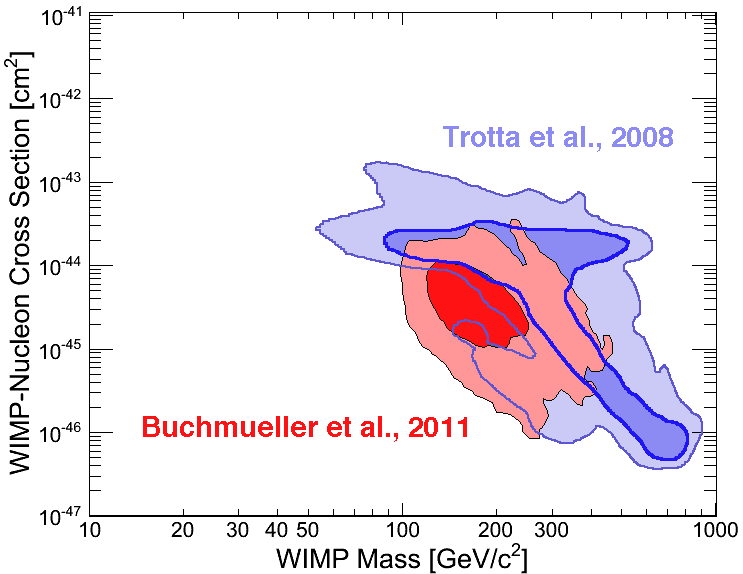
\includegraphics[width=0.475\linewidth]{plots/DarkMatter/wimp_expectation_modWithLabels.png}
\caption[The theoretical predictions for WIMP mass and spin-independent WIMP-nucleon scattering cross section with CMSSM]{The theoretical predictions for WIMP mass and spin-independent WIMP-nucleon scattering cross section with  constrained minimal supersymmetric extension to standard model (CMSSM)~\cite{LHC, Trotta}. Figure from Ref.~\cite{Marc}.}
\label{figCMSSMparameterSpace}
\end{figure}
%\end{floatingfigure}

%As time progresses, these rates begin to differ, the nature of which depends upon the particle�s annihilation cross section and mass. Once the temperature of the universe falls below the production threshold of this species, production ceases. Additionally, the expansion of the universe suppresses the annihilation rate; if this rate drops below the expansion rate then annihilation ceases as well, and a relic density of this particle will remain. The relic density of particle $\Chi$ depends upon is the thermally averaged
%total annihilation cross section multiplied by the velocity [$\sigma v$] as [29]:

%where mX , is the WIMP mass, nX is the number density, and ??v? is the thermally averaged
%total annihilation cross section multiplied by the velocity. In order for �X to have a value
%close to what we observe today, X must have a weak cross section [30], which already rules out most of the particles in the Standard Model.

